\section{Brugsscenarier}
\label{ParametreBrugsscenarier}
%
Da det tilstræbes at få et så naturligt scenarie, som muligt vil der ikke blive stilt en decideret opgave som testpersonerne skal løse men for at få de rejsende til, at sætte deres egne ord på oplevelsen af interaktionen med en social robot defineres der fire brugsscenarier, som anses for at forekomme naturligt i en lufthavn. De fire brugsscenarier henvender sig enten til at den rejsende skal finde gate information, toiletfaciliteter, indkøbsmuligheder eller forplejning. Det er derfor op til testpersonen selv at vælge, hvilket af de fire brugsscenarie, der gemmengåes. De fire brugsscenarier gengives i \textit{wireframe} designet i \textit{Marvel}, som præsenteres på \textit{Double}'s skærm. \textit{Wireframet} fremgår af \autoref{fig:SamledeWirefram}.
%
\begin{figure}[H]
\centering
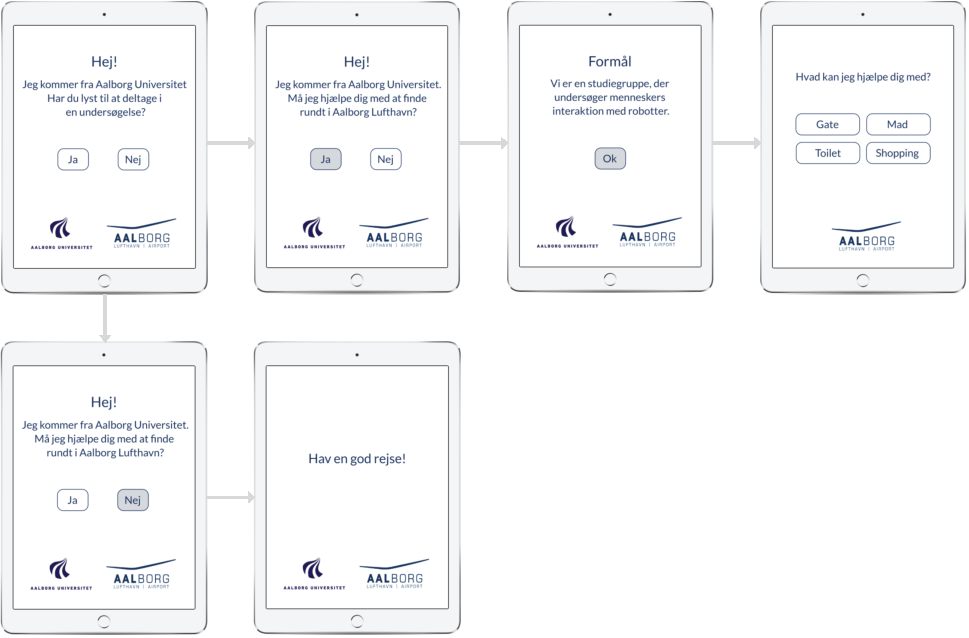
\includegraphics[width = \textwidth]{Figure/SamledeWirefram} 
\caption{Oversigt over de forskellige skærmbilleder i det samlede \textit{wirefram}, før der vælges brugsscenarie.}
\label{fig:SamledeWirefram}
\end{figure}
\noindent
%
På \autoref{fig:SamledeWirefram} illustreres de første skærmbilleder inden testpersonen vælger hvad robotten skal hjælpe dem med, jævnfør brugsscenariet. Derudover illustreres skærmbillederne i situationer hvor en rejsende ikke har lyst til at få hjælp af robotten. De fire forskellige brugsscenarier, som præsenteres afhængigt af testpersonen respons til spørgsmålet: \textit{Hvad kan jeg hjælpe dig med?}, indgår ikke på \autoref{fig:SamledeWirefram} men vil i de følgende afsnit blive præsenteret. 
  

\subsubsection*{Gate information}
%
Vælger testpersonerne at finde information om deres gate vil følgende skærmbilleder blivet præsenteret på skærmen, jævnfør \autoref{fig:GateInformation}. 
%
\begin{figure}[H]
\centering

\includegraphics[width = \textwidth]{Figure/GateInformation} 
\caption{Oversigt over de forskellige skærmbilleder, der anvendes i brugsscenariet: Gate information.}
\label{fig:GateInformation}
\end{figure}
\noindent
%
\autoref{fig:GateInformation} er blot et eksempel på hvilke skærmbilleder testpersonen præsenteres for, da den valgte gate er \textit{Gran Canaria}, vælges en af de andre destinationer vil navnet på den destination blive markeret og efterfølgende vil skærmbillederne være tilpasset denne destination. Vælger testpersonen at trykke på \textit{Udnyt tiden} bliver de spurgt hvad de har lyst til at lave mens de venter. Vælger testpersonen \textit{Shopping} vil skærmbillederne være de samme som illustreret på \autoref{fig:Indkoebsmuligheder}, hvor hvis testpersonen vælger \textit{Mad} vil skærmbillederne være de samme som illustreret på \autoref{fig:Forplejning}.  

\subsubsection*{Toiletfaciliteter}
%
Vælger testpersonerne at finde information om toiletfaciliteter vil følgende skærmbilleder blivet præsenteret på skærmen, jævnfør \autoref{fig:Toiletfaciliteter}. 
%
\begin{figure}[H]
\centering

\includegraphics[width = \textwidth]{Figure/Toiletfaciliteter} 
\caption{Oversigt over de forskellige skærmbilleder, der er specifikke for brugsscenariet: Toiletfaciliteter.}
\label{fig:Toiletfaciliteter}
\end{figure}
\noindent
%  
\subsubsection*{Indkøbsmuligheder}
%
Vælger testpersonerne at finde information om indkøbsmuligheder vil følgende skærmbilleder blivet præsenteret på skærmen, jævnfør \autoref{fig:Indkoebsmuligheder}. 
%
\begin{figure}[H]
\centering
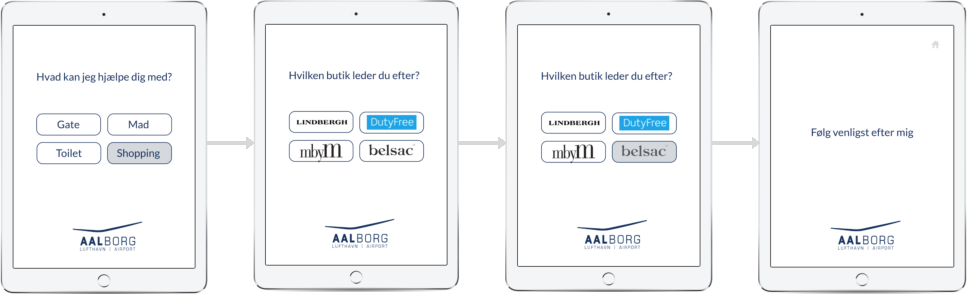
\includegraphics[width = \textwidth]{Figure/Indkoebsmuligheder} 
\caption{Oversigt over de forskellige skærmbilleder, der anvendes i brugsscenariet: Indkøbsmuligheder.}
\label{fig:Indkoebsmuligheder}
\end{figure}
\noindent
% 
\autoref{fig:Indkoebsmuligheder} er blot et eksempel på hvilke skærmbilleder testpersonen præsenteres for, da den valgte indkøbsmulighed er butikken \textit{Belsac}, vælges en af de andre muligheder vil navnet på den valgte butik blive markeret. 

\subsubsection*{Forplejning}
%
Vælger testpersonerne at finde information om forplejning vil følgende skærmbilleder blivet præsenteret på skærmen, jævnfør \autoref{fig:Forplejning}. 
%
\begin{figure}[H]
\centering
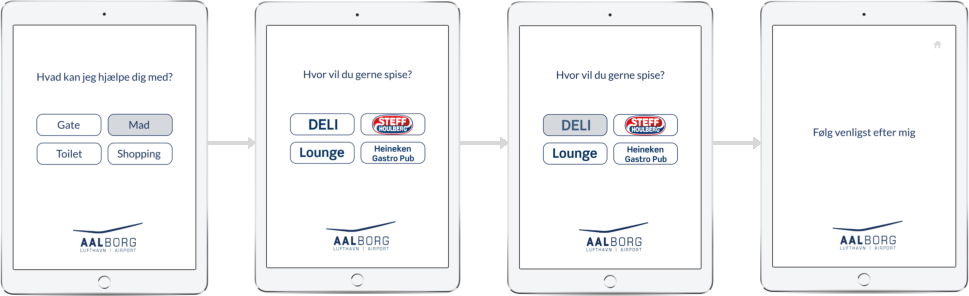
\includegraphics[width = \textwidth]{Figure/Forplejning} 
\caption{Oversigt over de forskellige skærmbilleder, der anvendes i brugsscenariet: Forplejning.}
\label{fig:Forplejning}
\end{figure}
\noindent
% 
\autoref{fig:Forplejning} er blot et eksempel på hvilke skærmbilleder testpersonen præsenteres for, da den valgte forplejning er \textit{DELI}, vælges en af de andre muligheder vil navnet på den valgte forplejning blive markeret. 

